\clearpage
\section{Blokové cyklické kódy}
\subsection{Čím se liší cyklický a blokový kód?}
Cyklický kód je určen namísto vytvářecí matice G vytvářecím mnohočlenem G(x).
Vytvářecí matice G některých lineárních kódů jdou převést součty mezi řádky do takového tvaru, že každý řádek obsahuje stejné prvky, pouze o jedno místo posunuté v jednom směru.

\subsection{Vysvětlete vazbu mezi vytvářecí maticí a vytvářecím mnohočlenem.}
Vytvářecí matice některých lineárních kódů lze převést lineárními kombinacemi
do takového tvaru, že každý řádek obsahuje stejný vektor, vždy o jeden symbol posunutý. 
Např.:\\ $G=\left[\begin{array}{ccccccc}
    1 & 1 & 0 & 1 & 0 & 0 & 0 \\
    0 & 1 & 1 & 0 & 1 & 0 & 0 \\
    0 & 0 & 1 & 1 & 0 & 1 & 0 \\
    0 & 0 & 0 & 1 & 1 & 0 & 1 
\end{array}
\right]$\\
Tento opakující se vektor $\left[\begin{array}{cccc} 1 & 1 & 0 & 1 \end{array}\right]$ je náš vytvářecí mnohočlen. Zbývá ho jen převést do polynomiálního tvaru:
$x^3+x^2+1$

\subsection{Matematický zapište proces kódování a dekódování cyklickým kódem.}
Definujeme si mnohočleny:
\begin{itemize}
    \item $P(x)$ - mnohočlen bloku nezabezpečené zprávy
    \item $G(x)$ - generující mnohočlen
    \item $M(x)$ - mnohočlen podílu, v zabezpečení se nevyužívá
    \item $R(x)$ - mnohočlen zbytku, z něj se tvoří zabezpečovací bity
    \item $F(x)$ - mnohočlen zabezpečené zprávy
    \item $J(x)$ - mnohočlen přijaté posloupnosti
    \item $S(x)$ - mnohočlen syndromu
    \item $E(x)$ - chybový mnohočlen
\end{itemize}
\subsubsection{Kódování}
$\frac{P(x)\cdot x^{(n-k)}}{G(x)}=M(x)_1+\frac{R(x)}{G(x)}$, $F(x)=P(x)\cdot x^{(n-k)}+R(x)$, $F(x)$ se odešle.
\subsubsection{Dekódování}
$\frac{J(x)}{G(x)}=M(x)_2+\frac{S(x)}{G(x)}$, Syndrom porovnáme s tabulkou syndromů vzniklou vydělením všech možných
chybových mnohočlenů vytvářecím mnohočlenem ($\frac{E(x)}{G(x)}=M(x)_3+\frac{S(x)}{G(x)}$)

\subsection{Uveďte některé cyklicky definované kódy.}
CRC kódy, cyklické kódy odvozené z Hammingova kódu, Fireův kód 

\subsection{Zapojení dekodéru cyklického detekčního kódu.}
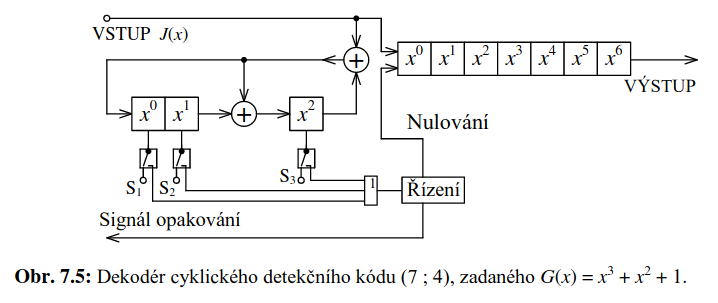
\includegraphics[width=16cm]{images/7_dekoder.png}

\subsection{Vysvětlete princip Meggitova dekodéru. Pro které kódy jej lze využít?}
Využít je lze pro kódy odvozené z Hammingova kódu.\\
Tabulka syndromů je tvořena od chybného bitu s nejvyšším řádem po chybný bit s nejnižším řádem.\\
Po načtení celého bloku je vypočten v dekodéru syndrom, po $n$ dalších kroků se na vstup dodávají jen nuly.\\
Pokud je chyba na prvním bitu (s nejvyšším řádem), bude vystupovat z děličky jako první. Syndrom 
pro první bit je známý.\\
Pokud je chyba na druhém bitu, po jednom kroku bude chybný bit připravený vystoupit z děličky, syndrom bude po tomto
kroku stejný jako v předešlém případě.\\
Stačí tedy kontrolovat, jestli syndrom v děličce odpovídá syndromu chyby prvního bitu a pokud ano, opravovat první bit
ve vstupní paměti. Dokud tento syndrom nemá tuto známou hodnotu, posouváme hodnoty v děličce i ve vstupní paměti 
vkládáním nul. (skripta, str. 109-110)

\subsection{Vysvětlete pojem Galoisovo těleso a uveďte, které kódy jej využívají?}
Pomocí prvků tohoto tělesa se uskutečňují operace spojené se zabezpečováním posloupnosti nezabezpečených signálových prvků. Galoisova tělesa GF (p$^r$). Zde $p$ je základ číselné soustavy (2) a $r$ odpovídá počtu zabezpečovacích prvků v mnohočlenu zabezpečené zprávy. Je tvořeno konečným počtem prvků n = p$^r$  a vzniklo rozšířením tzv. konečného tělesa Zp.

BCH kódy, Reed-Solomonovy (RS) kódy
